\section{Copyright Basics}

\begin{frame}
  \centering
  \href{https://www.youtube.com/watch?v=tHp3c9ziIq0}{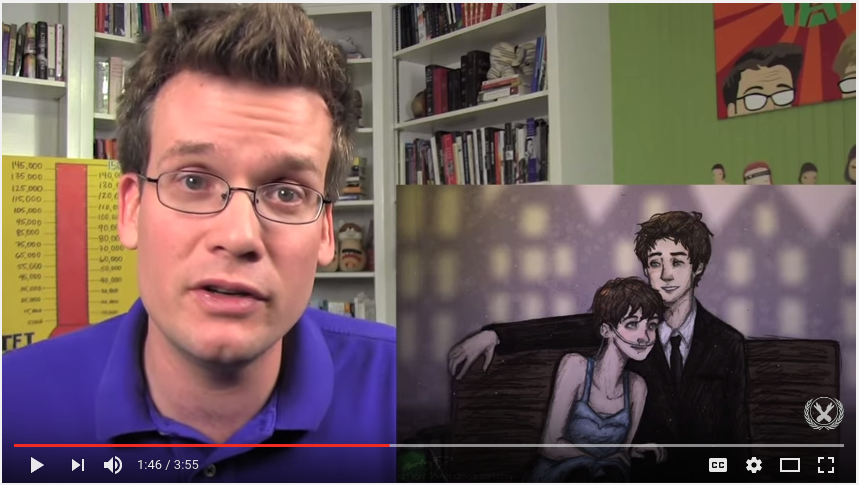
\includegraphics[scale=0.3]{images/john-green-tumblr-copyright-posters}}
\end{frame}

\begin{frame}
  \frametitle{What is Copyright?}

  \begin{itemize}
    \item Set of exclusive rights
    \item Granted to the author of a work for a limited period of time
    \item Meant to promote creativity
  \end{itemize}
\end{frame}

\begin{frame}
  \frametitle{Basis of Copyright in the U.S. Constitution}

  ``[The Congress shall have Power] To promote the Progress of Science and useful
  Arts, by securing for limited Times to Authors and Inventors the exclusive
  Right to their respective Writings and Discoveries.''

  \begin{flushright}
    ---Article I, Section 8, Clause 8
  \end{flushright}
\end{frame}

\begin{frame}
  \frametitle{Limitations on Exclusive Rights}

  \begin{itemize}
    \item Fair use/Fair dealing (17 U.S.C. § 107)
    \item First-sale doctrine (17 U.S.C. § 109)
    \item Backup copies of software (17 U.S.C. § 117)
    \item Mechanical licensing
    \begin{itemize}
      \item Automatically granted to record and publish covers of songs provided
      that royalties are paid
    \end{itemize}
    \item Works by the U.S. government cannot be copyrighted (17 U.S.C. § 105)
  \end{itemize}
\end{frame}
